% Created 2017-10-24 Tue 12:20
% Intended LaTeX compiler: pdflatex
\documentclass[11pt]{article}
\usepackage[utf8]{inputenc}
\usepackage{lmodern}
\usepackage[T1]{fontenc}
\usepackage{fixltx2e}
\usepackage{graphicx}
\usepackage{longtable}
\usepackage{float}
\usepackage{wrapfig}
\usepackage{rotating}
\usepackage[normalem]{ulem}
\usepackage{amsmath}
\usepackage{textcomp}
\usepackage{marvosym}
\usepackage{wasysym}
\usepackage{amssymb}
\usepackage{amsmath}
\usepackage[version=3]{mhchem}
\usepackage[numbers,super,sort&compress]{natbib}
\usepackage{natmove}
\usepackage{url}
\usepackage{minted}
\usepackage{underscore}
\usepackage[linktocpage,pdfstartview=FitH,colorlinks,
linkcolor=blue,anchorcolor=blue,
citecolor=blue,filecolor=blue,menucolor=blue,urlcolor=blue]{hyperref}
\usepackage{attachfile}
\usepackage[left=1in, right=1in, top=1in, bottom=1in, nohead]{geometry}
\usepackage{fancyhdr}
\usepackage{hyperref}
\usepackage{setspace}
\usepackage[labelfont=bf]{caption}
\usepackage{amsmath}
\usepackage{enumerate}
\usepackage[parfill]{parskip}
\date{Due: 10/24/2017}
\title{}
\begin{document}

\title{Computational Chemistry Homework 3}
\author{Jeonghyun Ko, Gray Laughlin, Yujia Wang}
\maketitle


Here is an example input deck for a HFS/6-31G calculation on NH\(_{\text{3}}\). This is a good starting template for the calculations below. You can also construct an input deck in Avogadro. Refer to the GAMESS manual for more information.

\begin{verbatim}
!   File created by the GAMESS Input Deck Generator Plugin for Avogadro
 $BASIS GBASIS=N31 NGAUSS=6 $END
 $CONTRL RUNTYP=ENERGY DFTTYP=SLATER $END

 $DATA 
Title
C1
N     7.0    -1.03363     0.80618     0.00000
H     1.0    -0.01363     0.80618     0.00000
H     1.0    -1.37362     1.64340    -0.47314
H     1.0    -1.37363     0.79732     0.96162
 $END
\end{verbatim}


\section{\texttt{GAMESS} vs. \texttt{FDA}}
\label{sec:orgfde3668}

Using \texttt{GAMESS}, perform a DFT/Hartree-Fock-Slater (\texttt{DFTTYP=SLATER}) calculation on an Ar atom using the 6-31G basis set.

\subsection{How many primitive Gaussians are included in this calculation? How many total basis functions? How do they divide between s, p, and d?}
\label{sec:orgd5d4049}

Input file of GAMESS for Ar 
\begin{verbatim}
 $BASIS GBASIS=N31 NGAUSS=6 $END
 $CONTRL RUNTYP=ENERGY DFTTYP=SLATER $END

 $DATA 
Title
C1
Ar    18.0    -3.86612     1.03789     0.00000
 $END
\end{verbatim}

Let's look at the log file. We used 13 primitive Gaussians.
\begin{minted}[frame=lines,fontsize=\scriptsize,linenos]{sh}
grep "GAUSSIAN BASIS FUNCTIONS" Ar/Ar.log
\end{minted}

\begin{verbatim}
NUMBER OF CARTESIAN GAUSSIAN BASIS FUNCTIONS =   13
\end{verbatim}

Because we used 6-31G Basis set, 6 gaussian functions are used for core shells and 3 and 1 gaussian functions are used for inner and outer regions of valance shells. See table below.

\begin{center}
\begin{tabular}{lrrr}
Orbital & Basis Sets & Primitive gauss functions & Total gauss functions\\
\hline
1s & 1 & 6 & 6\\
2s & 1 & 6 & 6\\
2p & 3 & 6 & 18\\
3s & 1 & 3 & 3\\
3p & 3 & 3 & 9\\
3s+ & 1 & 1 & 1\\
3p+ & 3 & 1 & 3\\
\hline
Total & 13 &  & 46\\
\end{tabular}
\end{center}

\subsection{How many SCF iterations does the calculation take to converge?}
\label{sec:org8d38e84}

Let's look at the log file again. 12 iterations are required to reach convergence.

\begin{minted}[frame=lines,fontsize=\scriptsize,linenos]{sh}
grep "ITER" Ar/Ar.dat
\end{minted}

\begin{center}
\begin{tabular}{lll}
E(R-SLATER)=     -524.4520526614 & E(NUC)=    0.0000000000 & 12 ITERS\\
\end{tabular}
\end{center}

\subsection{What is the final calculated HFS/6-31G energy of the atom?}
\label{sec:orgcd32e63}

The final HFS/6-31G energy: -524.452 Hartree.

\subsection{What are the identities (1s, 2p, etc.) and energies of the occupied atomic orbitals?}
\label{sec:org9bd422a}

E\_FDA values are from HW2.

\begin{center}
\begin{tabular}{lrr}
Orbital & E\(_{\text{GAMESS}}\) (Hartree) & E\(_{\text{FDA}}\) (Hartree)\\
\hline
1s & -113.6768 & -116.9366\\
2s & -10.7172 & -11.6037\\
2p & -8.3677 & -9.2721\\
3s & -0.8218 & -1.1022\\
3p & -0.3222 & -0.5735\\
3s+ & 0.4316 & \\
3p+ & 0.5206 & \\
\end{tabular}
\end{center}

\subsection{Compare your computed total energy and atomic orbital energies with those you got from Homework 2 using the fda code for Ar.}
\label{sec:orgf349d4d}

The total energy from FDA is -526.8275 Hartree. Compared to HFSs/6-31G energy (-254.425 Hartree), FDA shows slightly lower total energy.

\section{The Generalized Gradient Approximation}
\label{sec:orgafc2456}

The generalized gradient approximation (GGA) is an improvement on Hartree-Fock-Slater that gives a nice balance between accuracy and computational expense. Using \texttt{GAMESS}, perform a single point calculation (\texttt{RUNTYP=ENERGY}) on the bent triatomic SO\(_{\text{2}}\) using the GGA (\texttt{DFTTYP=PBE}) and PC1 basis set (\texttt{GBASIS=PC1}, \texttt{ISPHER=1}; no \texttt{NGAUSS} flag needed). Guess appropriate bond lengths and angle. Be sure to report your input file for your calculation.

\subsection{What is the spin multiplicity of SO\(_{\text{2}}\)? (Recall, the spin multiplicity is 2S +1, where S = 1/2 for one unpaired electron, S = 1 for two unpaired electrons, and so on).}
\label{sec:org8f8e502}

The spin multiplicity for SO\(_{\text{2}}\) is 2 * 0 + 1 = 1. 

\subsection{How many basis functions are in this calculation?}
\label{sec:orgb3a24c5}

Let's look at the log file. We used 49 primitive Gaussians.
\begin{minted}[frame=lines,fontsize=\scriptsize,linenos]{sh}
grep "GAUSSIAN BASIS FUNCTIONS" SO2/SO2.log
\end{minted}

\begin{verbatim}
NUMBER OF CARTESIAN GAUSSIAN BASIS FUNCTIONS =   49
\end{verbatim}

\subsection{How many SCF cycles does it take to converge?}
\label{sec:org6cc14ec}

It takes 22 SCF cycles to converge.

\begin{minted}[frame=lines,fontsize=\scriptsize,linenos]{sh}
grep "ITER" SO2/SO2.dat
\end{minted}

\begin{center}
\begin{tabular}{lll}
E(R-PBE)=     -548.2342329889 & E(NUC)=  109.8468077125 & 22 ITERS\\
\end{tabular}
\end{center}

\subsection{What SCF algorithm does the code use?}
\label{sec:orgbaba4ed}

The code uses the DIIS algorithm.

See log file. we can see "DIIS = T"

\subsection{What is the final total energy of the molecule?}
\label{sec:org7bc710a}

The final total energy is -548.234 Hartree

\begin{minted}[frame=lines,fontsize=\scriptsize,linenos]{sh}
grep "TOTAL ENERGY = " SO2/SO2.log
\end{minted}

\begin{verbatim}
TOTAL ENERGY =    -548.2342329889
\end{verbatim}

\subsection{How many occupied orbitals does the molecule have? What are the energies of the HOMO and LUMO?}
\label{sec:org0fd26a8}

There are 16 occupied orbitals.

\begin{minted}[frame=lines,fontsize=\scriptsize,linenos]{sh}
grep "NUMBER OF OCCUPIED" SO2/SO2.log
\end{minted}

\begin{center}
\begin{tabular}{llllllrr}
NUMBER & OF & OCCUPIED & ORBITALS & (ALPHA) & = & 16 & \\
NUMBER & OF & OCCUPIED & ORBITALS & (BETA & ) & = & 16\\
\end{tabular}
\end{center}


HOMO: -0.2826 Hartree (16th)

LUMO: -0.1472 Hartree (17th)

\subsection{What is the final dipole moment?}
\label{sec:orgce0b67b}

The final dipole moment is 1.453 debyes

\subsection{What are the Mulliken gross charges on the S and O atoms?}
\label{sec:org874f83a}

The Mulliken charges are tabulated below.

\begin{center}
\begin{tabular}{lr}
ATOM & CHARGE\\
\hline
S & 0.570174\\
O & -0.296290\\
O & -0.273884\\
\end{tabular}
\end{center}

\subsection{Plot out the electrostatic potential of SO\(_{\text{2}}\). Which end of the molecule is electrophilic and which is nucleophilic?}
\label{sec:org86115f5}

The electrostatic potential can be plotted by using Avogadro.

\begin{center}
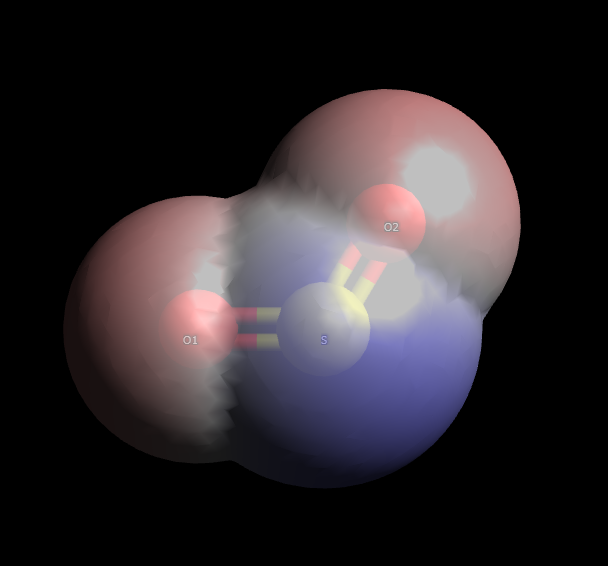
\includegraphics[width=4in]{./SO2/SO2.png}
\end{center}

\section{Geometry Optimization of SO\(_{\text{2}}\)}
\label{sec:orgdbc0177}

\subsection{Do a series of calculations in which you vary the S–O distances and O–S–O angle over a regular grid of values. Approximate the combination of values that give the lowest energy.}
\label{sec:org25d5d35}

Molecular energies were calculated using Gaussian B3LYP functional and 6-31G(d) basis set:

\begin{center}
\begin{tabular}{lrrrrr}
Energy (Ha) & 1.35(\AA{}) & 1.45(\AA{}) & 1.50(\AA{}) & 1.55(\AA{}) & 1.65(\AA{})\\
\hline
105\textdegree{} & -548.531 & -548.574 & -548.574 & -548.565 & -548.529\\
115\textdegree{} & -548.548 & -548.586 & -548.584 & -548.573 & -548.535\\
120\textdegree{} & -548.550 & \textbf{-548.587} & -548.585 & -548.573 & -548.534\\
125\textdegree{} & -548.549 & -548.585 & -548.583 & -548.571 & -548.532\\
135\textdegree{} & -548.538 & -548.574 & -548.572 & -548.561 & -548.523\\
\end{tabular}
\end{center}

As shown in the table, the combination of values that give the lowest energy is S–O distance = 1.45 \AA{} and O–S–O angle = 120\textdegree{}.

\subsection{A geometry optimization is a faster way to find the optimal geometry of a molecule. Perform a geometry optimization on SO\(_{\text{2}}\) using the same computational model as above. What are the optimal S–O distances and O–S–O angle?}
\label{sec:org83a1758}

Geometry optimization was done using Gaussian B3LYP functional and 6-31G(d) basis set (\url{./SO2.txt}): the optimal S–O distances are 1.46 \AA{} and O–S–O angle is 119\textdegree{}. We got pretty close results using the rough scan.

\section{Other Molecules}
\label{sec:orgadc0258}

Oxygen makes bonds with lots of things. Fill out the table below by doing an appropriate set of calculations:

Geometry optimization was done using Gaussian B3LYP functional and 6-31G(d) basis set:

\begin{center}
\begin{tabular}{lrrrrl}
AO\(_{\text{2}}\) & A-O (\AA{}) & O-A-O (\textdegree{}) & Spin Multiplicity & Dipole Moment (e\AA{}) & Mulliken Charge\\
\hline
CO\(_{\text{2}}\) \url{./CO2.txt} & 1.169 & 180 & 1 & 0 & C: 0.72, O: -0.36\\
NO\(_{\text{2}}\) \url{./NO2.txt} & 1.203 & 133.84 & 2 & 0.32 & N: 0.48, O: -0.24\\
SiO\(_{\text{2}}\)\url{./SiO2.txt} & 1.520 & 180 & 1 & 0 & Si: 0.95, O: -0.48\\
SO\(_{\text{2}}\) \url{./SO2.txt} & 1.463 & 119.08 & 1 & 1.78 & S: 0.82, O: -0.41\\
\end{tabular}
\end{center}
\end{document}